\chapter{Implementation Details}
\label{chap:implementation}

This chapter provides detailed descriptions of the core algorithms and implementation techniques used in the {\name} system.

\section{Core Algorithm Implementation}
\label{sec:core_algorithms}

\subsection{Web Structure Extraction Algorithm}

The web structure extraction process follows a systematic approach to capture DOM elements and their associated CSS properties.

% Algorithm environment commented out due to missing packages
% \begin{algorithm}[H]
% \caption{Web Structure Extraction}
% \label{alg:web_extraction}
% \begin{algorithmic}[1]
% \REQUIRE URL list $U$, Analysis levels $L$
% \ENSURE Structured data $D$ with DOM elements and CSS properties
% \STATE Initialize WebDriver with Chrome configuration
% \FOR{each $url \in U$}
%     \STATE Load $url$ in browser with error handling
%     \STATE Extract DOM tree structure
%     \FOR{each $level \in L$}
%         \STATE Collect elements at depth $level$
%         \STATE Extract computed CSS styles
%         \STATE Store element attributes and properties
%     \ENDFOR
%     \STATE Generate unique identifiers for elements
%     \STATE Save structured data to $D$
% \ENDFOR
% \RETURN $D$
% \end{algorithmic}
% \end{algorithm}

\textbf{Algorithm 1: Web Structure Extraction}
\begin{enumerate}
\item \textbf{Input:} URL list $U$, Analysis levels $L$
\item \textbf{Output:} Structured data $D$ with DOM elements and CSS properties
\item Initialize WebDriver with Chrome configuration
\item For each $url \in U$:
\begin{enumerate}
    \item Load $url$ in browser with error handling
    \item Extract DOM tree structure
    \item For each $level \in L$:
    \begin{enumerate}
        \item Collect elements at depth $level$
        \item Extract computed CSS styles
        \item Store element attributes and properties
    \end{enumerate}
    \item Generate unique identifiers for elements
    \item Save structured data to $D$
\end{enumerate}
\item Return $D$
\end{enumerate}

The extraction algorithm processes websites at multiple DOM levels, capturing both structural hierarchy and styling information. Each element receives a unique identifier generated using timestamp and random components to ensure uniqueness across processing sessions.

\subsection{HDBSCAN Clustering Implementation}

The clustering algorithm utilizes HDBSCAN (Hierarchical Density-Based Spatial Clustering of Applications with Noise) for grouping structurally similar elements.

% Algorithm environment commented out due to missing packages
% \begin{algorithm}[H]
% \caption{HDBSCAN Clustering with Optimization}
% \label{alg:hdbscan_clustering}
% \begin{algorithmic}[1]
% \REQUIRE Structured data $D$, Parameter ranges $P$
% \ENSURE Clustered elements $C$ with optimal parameters
% \STATE Extract feature vectors from $D$
% \STATE Normalize features using StandardScaler
% \STATE $best\_score \gets 0$, $best\_params \gets \emptyset$
% \FOR{each parameter combination $p \in P$}
%     \STATE Apply HDBSCAN clustering with parameters $p$
%     \STATE Compute DBCV score for validation
%     \IF{DBCV score $>$ $best\_score$}
%         \STATE $best\_score \gets$ DBCV score
%         \STATE $best\_params \gets p$
%     \ENDIF
% \ENDFOR
% \STATE Apply clustering with $best\_params$
% \STATE Reassign outliers to nearest clusters using Euclidean distance
% \RETURN $C$
% \end{algorithmic}
% \end{algorithm}

\textbf{Algorithm 2: HDBSCAN Clustering with Optimization}
\begin{enumerate}
\item \textbf{Input:} Structured data $D$, Parameter ranges $P$
\item \textbf{Output:} Clustered elements $C$ with optimal parameters
\item Extract feature vectors from $D$
\item Normalize features using StandardScaler
\item Set $best\_score \gets 0$, $best\_params \gets \emptyset$
\item For each parameter combination $p \in P$:
\begin{enumerate}
    \item Apply HDBSCAN clustering with parameters $p$
    \item Compute DBCV score for validation
    \item If DBCV score $>$ $best\_score$:
    \begin{enumerate}
        \item $best\_score \gets$ DBCV score
        \item $best\_params \gets p$
    \end{enumerate}
\end{enumerate}
\item Apply clustering with $best\_params$
\item Reassign outliers to nearest clusters using Euclidean distance
\item Return $C$
\end{enumerate}

The clustering implementation includes sophisticated parameter optimization through grid search over minimum cluster sizes and cluster selection epsilon values. The DBCV validation metric ensures high-quality clusters while the outlier reassignment strategy minimizes noise in the final results.

\section{Dual-Layer Caching System}
\label{sec:caching_system}

The caching system implements a sophisticated dual-layer approach to optimize performance.

\begin{figure}[h]
\centering
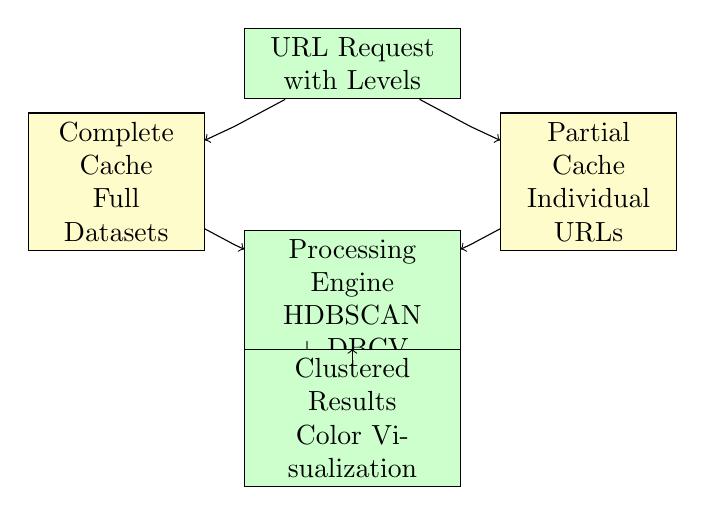
\begin{tikzpicture}[
    box/.style={rectangle, draw, fill=green!20, text width=2.5cm, text centered, minimum height=0.8cm},
    cache/.style={rectangle, draw, fill=yellow!20, text width=2cm, text centered, minimum height=0.6cm}
]
    \node[box] (request) at (0,2.5) {URL Request\\with Levels};
    \node[cache] (complete) at (-3,1) {Complete Cache\\Full Datasets};
    \node[cache] (partial) at (3,1) {Partial Cache\\Individual URLs};
    \node[box] (processing) at (0,-0.5) {Processing Engine\\HDBSCAN + DBCV};
    \node[box] (output) at (0,-2) {Clustered Results\\Color Visualization};
    
    \draw[->] (request) -- (-1.5,1.7) -- (complete);
    \draw[->] (request) -- (1.5,1.7) -- (partial);
    \draw[->] (complete) -- (-1.5,0.2) -- (processing);
    \draw[->] (partial) -- (1.5,0.2) -- (processing);
    \draw[->] (processing) -- (output);
\end{tikzpicture}
\caption{Dual-Layer Caching Architecture}
\label{fig:cache_architecture}
\end{figure}

The caching system provides optimization through:

\begin{itemize}
\item \textbf{Individual URL Caching.} Stores processed DOM and CSS data for each URL individually, enabling reuse when the same URL appears in different analysis combinations.
\item \textbf{Intelligent Reuse.} Previously processed URLs can be retrieved from cache while new URLs are processed and added to the cache for future use.
\end{itemize}

\section{Feature Extraction and Processing}
\label{sec:feature_extraction}

\subsection{CSS Property Normalization}

The system handles various CSS property types through specialized normalization:

\begin{itemize}
\item \textbf{Pixel Values.} Converted to numerical format with special handling for 'auto' and percentage values.
\item \textbf{Color Values.} RGB and RGBA values converted to HSL color space for better clustering.
\item \textbf{String Attributes.} Categorical values mapped to numerical indices in a consistent vector space.
\item \textbf{Multi-value Properties.} Properties like margins and paddings decomposed into individual components.
\end{itemize}

\subsection{Vector Space Construction}

Elements are represented as feature vectors combining:

\begin{itemize}
\item Normalized CSS property values
\item Structural position information
\item Element type classifications
\item Text content characteristics
\end{itemize}

The resulting vectors undergo StandardScaler normalization before clustering to ensure equal importance of all features.

\section{API Implementation}
\label{sec:api_implementation}

\subsection{RESTful Endpoint Design}

The Flask API provides comprehensive endpoints for system interaction:

\begin{lstlisting}[language=Python]
@app.route('/process-urls', methods=['POST'])
def process_urls():
    data = request.json
    urls = data.get('urls', [])
    levels = data.get('levels', [])
    mode = data.get('mode', 0)
    results = process_urls_from_api(urls, levels, mode)
    return jsonify(results)

@app.route('/cache/stats', methods=['GET'])
def get_cache_stats():
    stats = cache_manager.get_cache_stats()
    return jsonify({"status": "success", "data": stats})
\end{lstlisting}

\subsection{Request Validation}

All API endpoints implement comprehensive input validation:

\begin{itemize}
\item URL format validation using regular expressions
\item Parameter range checking for levels and processing modes
\item Request size limits to prevent resource exhaustion
\item Content-type verification for security
\end{itemize}

\section{Frontend Implementation}
\label{sec:frontend_implementation}

The frontend implementation realizes the user interface design described in Section~\ref{sec:user_interface}, providing a comprehensive web-based interface for all system functionality.

\subsection{React Component Architecture}

The frontend follows a modular component structure with the main URLChipForm component implementing the tabbed interface shown in Figure~\ref{fig:ui_main_interface}:

\begin{lstlisting}[language=JavaScript]
const URLChipForm = ({ darkMode, onThemeChange }) => {
    const [urls, setUrls] = useState([]);
    const [selectedLevels, setSelectedLevels] = useState([]);
    const [result, setResult] = useState(null);
    
    const handleRun = async () => {
        const response = await fetch("http://localhost:5000/process-urls", {
            method: 'POST',
            headers: { 'Content-Type': 'application/json' },
            body: JSON.stringify({ urls, levels: selectedLevels })
        });
        const data = await response.json();
        setResult(data);
    };
    
    return (
        // Component JSX
    );
};
\end{lstlisting}

\subsection{Performance Optimization}

The application uses React hooks for state management and optimization:

\begin{itemize}
\item \textbf{useState} for component-level state management
\item \textbf{useEffect} for side effects and data fetching
\item \textbf{useMemo} for expensive computations
\item \textbf{Custom hooks} for reusable logic abstraction
\end{itemize}

\section{Project Orchestration}
\label{sec:project_orchestration}

The system uses mprocs for multi-process orchestration, coordinating the execution of multiple services simultaneously. The mprocs.yml configuration file defines four main processes:

\begin{itemize}
\item \textbf{ReactApp:} Frontend development server (port 3000)
\item \textbf{PythonApi:} Flask API backend (port 5000)
\item \textbf{BackendApiNodeServer:} Static file server (port 5005)
\item \textbf{PythonApiTests:} Automated testing process
\end{itemize}

This orchestration approach enables developers to start all system components with a single command, streamlining the development and deployment process. 